% =====================================================================
%  chunk c11 —— 植田一石《ホモロジー的ミラー対称性》
%  第 31–34 节，原书 p043–p049（p049 末尾含「参考文献」标题及首 3 条）
%  编号公式 53 条（p043: 12，p044: 5，p045: 7，p046: 8，p047: 3，p048: 8，p049: 10）
%  图：图 31.1–31.4（p044×3、p045×1），图 32.1–32.2（p046）
% =====================================================================
% [Tutor Note: 公式条数以页面图像上实际印出的编号公式为准（不凑数）。
%  work/tags_bypage.txt 对 p043–p049 的命中数为 12/5/7/8/3/8/11，其中 p049 的第 11 个
%  是正文交叉引用「(33.10) から」，实际编号公式 10 条；其余各页命中数与实际条数一致。
%  合计 53 条，已逐页比对图像核对，未增补、未重排。]
%
% [Tutor Note: 关于 p049 末尾的参考文献。原书「参考文献」标题与前 3 条
%  （[AAE+13]、[ABC+09]、[Aboa]）印在 p049，属本 chunk 页范围，故此处照录；
%  （Lead 已处理：这 3 条与标题已并入 c12.tex，c11 末尾不再重复。）]

\section{$A_1$ 奇点}

对复数 $a_0, a_1$，由
\begin{equation}
Y := \left\{(z,u,v) \in \C^3 \mid uv = (z-a_0)(z-a_1)\right\} \tag{31.1}
\end{equation}
定义的 $\C^3$ 的超曲面，在 $a_0 = a_1$ 时于 $(z,u,v) = (a_0,0,0)$ 处具有 $A_1$ 奇点，而 $a_0 \ne a_1$ 时非奇异。取定一组相异的 $a_0, a_1 \in \C^{\times}$，考虑 $Y$ 的开子流形
\begin{equation}
Y^0 := \left\{(z,u,v) \in Y \mid z \ne 0\right\} \tag{31.2}
\end{equation}
通过把 Kähler 形式与全纯体积形式定义为
\begin{equation}
\omega = \frac{1}{2\sqrt{-1}}\left(\frac{dz \wedge d\bar z}{2\pi|z|^{2}} + du \wedge d\bar u + dv \wedge d\bar v\right)\bigg|_{Y^0}, \tag{31.3}
\end{equation}
\begin{equation}
\Omega = d\log z \wedge d\log u\bigg|_{Y^0} \tag{31.4}
\end{equation}
便使 $Y^0$ 成为近 Calabi--Yau 流形。$Y^0$ 通过
\begin{equation}
S^1 \ni \ee^{\sqrt{-1}\theta} : (z,u,v) \mapsto \left(z, \ee^{\sqrt{-1}\theta}u, \ee^{-\sqrt{-1}\theta}v\right) \tag{31.5}
\end{equation}
具有自然的 $S^1$ 作用；这是一个以
\begin{equation}
\mu : Y^0 \to \R,\quad (z,u,v) \mapsto \frac{1}{2}(|u|^2 - |v|^2) \tag{31.6}
\end{equation}
为 Hamilton 函数的 Hamilton 作用，并且保持全纯体积形式 $\Omega$。$\mu$ 的正则值处的辛商自然同构于赋以适当辛形式的 $z$ 平面，而 $s: z \mapsto \log|z|$ 给出其上的特殊拉格朗日纤维化；因此由定理 30.3，
\begin{equation}
\pi = (s,\mu) : Y^0 \to \R^2,\quad (z,u,v) \mapsto \left(\log|z|, \frac{1}{2}(|u|^2 - |v|^2)\right) \tag{31.7}
\end{equation}
给出 $Y^0$ 的特殊拉格朗日纤维化。在 $b = (s,\mu) \in \R^2$ 处 $\pi$ 的纤维由
\begin{equation}
L_b := \left\{(z,u,v) \in \C^3 \mid uv = (z-a_0)(z-a_1),\ |z| = r,\ |u|^2 - |v|^2 = 2\mu\right\} \tag{31.8}
\end{equation}
给出。

对任意 $b$，$z$ 投影 $p: (z,u,v) \mapsto z$ 给出从 $L_b$ 到 $\{z \in \C^\times \mid |z| = r\} \cong S^1$ 的满射。注意在 $L_b$ 中固定 $z$ 时 $|u|$ 与 $|v|$ 也随之固定，便知此投影的纤维在 $z \ne a_0, a_1$ 时同胚于 $S^1$，而在 $z = a_0$ 或 $z = a_1$ 时成为一点。因此 $\pi$ 的判别式集合为 $\Gamma := \{(s_0,0),(s_1,0)\}$，这些点上的纤维是把 $S^1 \times S^1$ 的一个圈收缩为一点所得的空间。其中对 $i = 0,1$ 置 $s_i := \log|a_i|$。

光滑纤维 $L_b$ 的一次同调群 $H_1(L_b;\Z)$ 由 $z$ 投影的截面与纤维生成。当 $L_b$ 中嵌入有向圆周时，它所属的同调类由其在 $z$ 平面、$u$ 平面及 $v$ 平面上的投影绕原点的卷绕数 $\varphi_z, \varphi_u$ 及 $\varphi_v$ 所指定。
\begin{equation}
uv = (z-a_0)(z-a_1) \tag{31.9}
\end{equation}
由此，把 $\R^2$ 分成三个区域
\begin{align}
U_0 &:= \left\{(s,\mu) \in \R^2 \mid s < s_0\right\}, \tag{31.10}\\
U_1 &:= \left\{(s,\mu) \in \R^2 \mid s_0 < s < s_1\right\}, \tag{31.11}\\
U_2 &:= \left\{(s,\mu) \in \R^2 \mid s_1 < s\right\} \tag{31.12}
\end{align}
及其补集，则这些卷绕数满足
\begin{equation}
\varphi_u + \varphi_v = \begin{cases}
0 & \text{在 } U_0 \text{ 上}\\
\varphi_z & \text{在 } U_1 \text{ 上}\\
2\varphi_z & \text{在 } U_2 \text{ 上}
\end{cases} \tag{31.13}
\end{equation}

\begin{figure}[htbp]
  \centering
  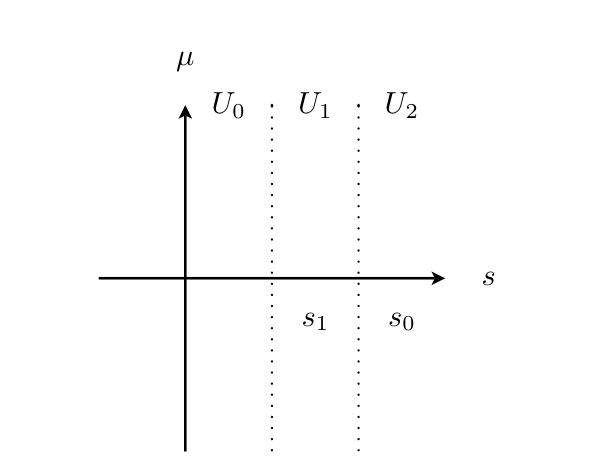
\includegraphics[width=0.5\textwidth]{figures/fig31.1.png}
  \figtitle{31.1}{底空间上的判别式与墙}
\end{figure}

\begin{figure}[htbp]
  \centering
  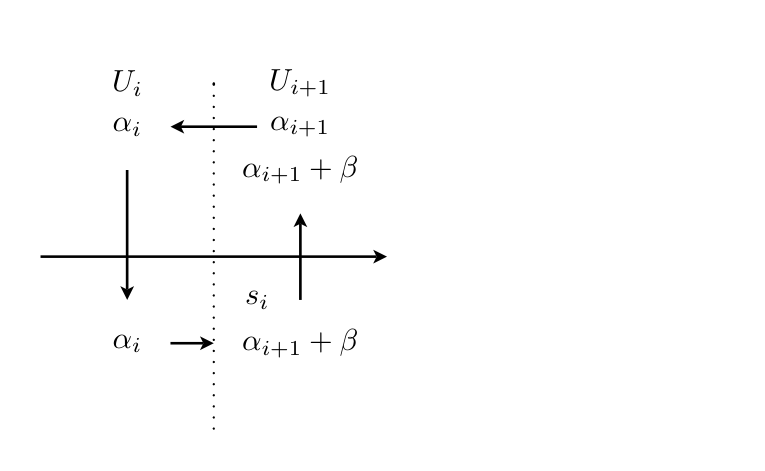
\includegraphics[width=0.55\textwidth]{figures/fig31.2.png}
  \figtitle{31.2}{单值}
\end{figure}

\begin{figure}[htbp]
  \centering
  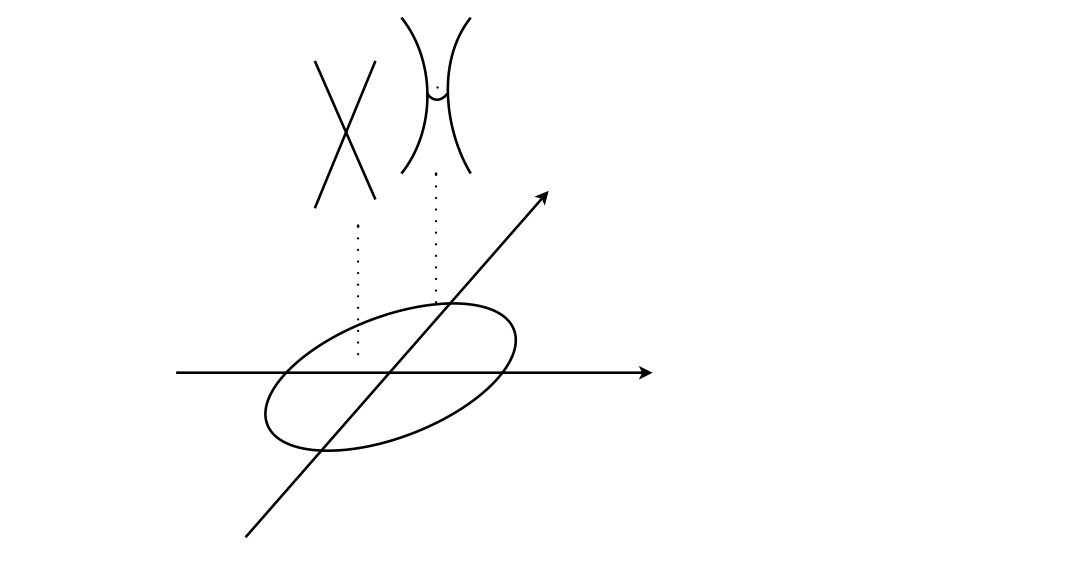
\includegraphics[width=0.6\textwidth]{figures/fig31.3.png}
  \figtitle{31.3}{拉格朗日环面}
\end{figure}

在 $b \in U_i$ 处 $H_1(L_b;\Z)$ 的基由
\begin{equation}
\alpha_i := \left\{(z,u,v) \in L_b \;\middle|\; z = r\ee^{2\pi\sqrt{-1}\theta}\text{，且 } u \text{ 与 } v \text{ 绕原点的卷绕数分别为 } 0 \text{ 与 } i\right\}, \tag{31.14}
\end{equation}
\begin{equation}
\beta := \left\{(z,u,v) \in L_b \;\middle|\; z = r,\ u = |u|\cdot\ee^{2\pi\sqrt{-1}\theta},\ v = |v|\cdot\ee^{-2\pi\sqrt{-1}\theta}\right\} \tag{31.15}
\end{equation}
给出。注意在 $\beta$ 的定义中，固定 $z$ 时 $|u|$ 与 $|v|$ 是被固定的。$\alpha_i$ 依赖于 $i$，而 $\beta$ 不依赖于 $i$。

同调类 $\alpha \in H_1(L_b;\Z)$ 对一切 $b \in \R^2 \setminus \Gamma$ 都有定义，而 $\beta_i$ 在 $\Gamma$ 的周围具有单值。若把 $\beta_i$ 从 $U_i$ 通过 $\mu > 0$ 的区域移动到 $U_{i+1}$，则这里恒有 $u > 0$，同时 $z = a_i$ 处 $v = 0$。因此可知，在此操作下 $\varphi_u$ 不变，而 $\varphi_v$ 只增加 $1$。同样地，若把 $\beta_i$ 从 $U_i$ 通过 $\mu < 0$ 的区域移动到 $U_{i+1}$，则 $\varphi_u$ 只增加 $1$，而 $\varphi_v$ 保持不变。

$\alpha_i$ 与 $\beta$ 对应的卷绕数 $(\varphi_z, \varphi_u, \varphi_v)$ 分别为 $(1,0,i)$ 及 $(0,1,-1)$，而在 $s_i \in \Gamma$ 的周围圈的单值，可由图 31.2 读出为
\begin{align}
\alpha_{i+1} &\mapsto \alpha_{i+1} + \beta \tag{31.16}\\
\beta &\mapsto \beta \tag{31.17}
\end{align}

\begin{figure}[htbp]
  \centering
  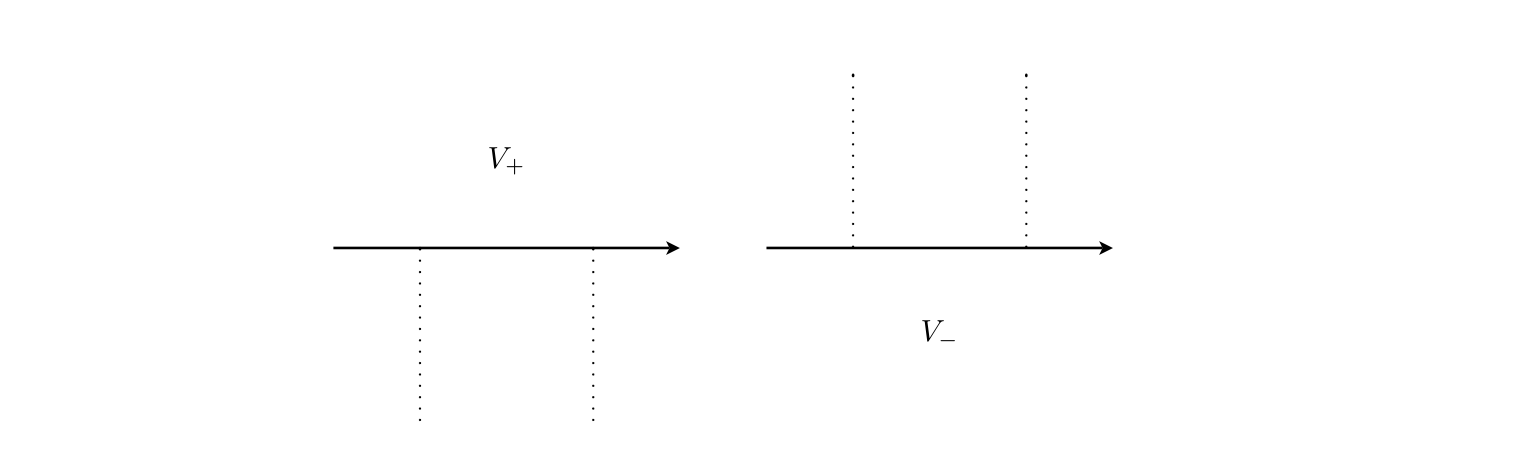
\includegraphics[width=0.6\textwidth]{figures/fig31.4.png}
  \figtitle{31.4}{两个开集}
\end{figure}

从判别式集合 $\Gamma$ 沿单值不变的方向延伸所得的直线 $\{s = s_i\}$ 称为墙（wall）。$\R^2 \setminus \Gamma$ 可用除去墙的下半与上半所得的集合
\begin{align}
V_+ &= \R^2 \setminus \left\{(s_i,\mu) \in \R^2 \mid i = 0,1,\ \mu \le 0\right\}, \tag{31.18}\\
V_- &= \R^2 \setminus \left\{(s_i,\mu) \in \R^2 \mid i = 0,1,\ \mu \ge 0\right\} \tag{31.19}
\end{align}
写成 $V_+ \cup V_-$。$V_+ \cap V_- = U_0 \sqcup U_1 \sqcup U_2$，而 $B_0$ 的仿射结构由把 $V_+$ 与 $V_-$ 的标准仿射结构按转换函数
\begin{equation}
\phi_{V_-,V_+}(s,\mu) = \begin{cases}
(s,\mu) & (s,\mu) \in U_0\\
(s,s+\mu) & (s,\mu) \in U_1\\
(s,2s+\mu) & (s,\mu) \in U_2
\end{cases} \tag{31.20}
\end{equation}
黏合而得。

在 $(s_0,0)$ 与 $(s_1,0)$ 处 $B$ 的奇点称为焦点-焦点奇点（focus-focus singularity）。由 Gauss--Bonnet 型定理可知：容许至多带焦点-焦点奇点的热带仿射结构的紧 $2$ 维流形只有球面、实射影平面、环面及 Klein 瓶这 $4$ 种；且各情形下焦点-焦点奇点的个数必须分别为 $24$ 个、$12$ 个、$0$ 个、$0$ 个 [LS10]。对应的辛流形分别是 K3 曲面、Enriques 曲面、环面上的环面丛、Klein 瓶上的环面丛。

\section{热带几何}

无奇点的紧热带仿射流形只限于仿射空间对离散群的商空间，因此要构造其他例子就无法回避奇点。置判别式集合的补集为 $B^{\mathrm{sm}} := B \setminus \Gamma$，则 $TB^{\mathrm{sm}}/T_{\Z}B^{\mathrm{sm}}$ 具有半平坦复结构；但为把它延拓到判别式集合，据信需要由全纯圆盘计数给出的瞬子修正 [Fuk05]。这种瞬子修正是非局部的，具体计算一般极为困难。

另一方面，对给定的热带仿射流形，可以考察半平坦复结构的自然单参数族
\begin{equation}
X_\epsilon(B_0) := TB_0/tT_{\Z}B_0 \tag{32.1}
\end{equation}
例如当 $B = B^{\mathrm{sm}} := \R/r\Z$ 是半径为 $r$ 的圆周时，对应的单参数族为
\begin{align}
X_\epsilon(B) &:= TS^1/tT_{\Z}S^1 \tag{32.2}\\
&= \C/\left(t\Z + \sqrt{-1}r\Z\right) \tag{32.3}\\
&\cong \C/\left(\Z + t^{-1}r\sqrt{-1}\Z\right) \tag{32.4}
\end{align}
可见在令 $\epsilon$ 趋于 $0$ 的极限下周期趋于无穷大。

\begin{figure}[htbp]
  \centering
  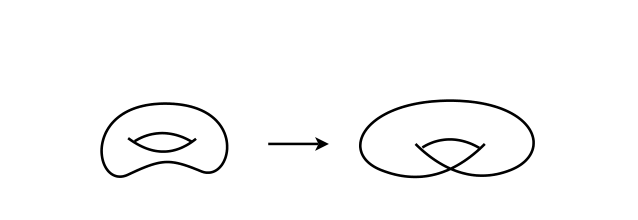
\includegraphics[width=0.4\textwidth]{figures/fig32.1.png}
  \figtitle{32.1}{代数几何意义下的退化}
\end{figure}

\begin{figure}[htbp]
  \centering
  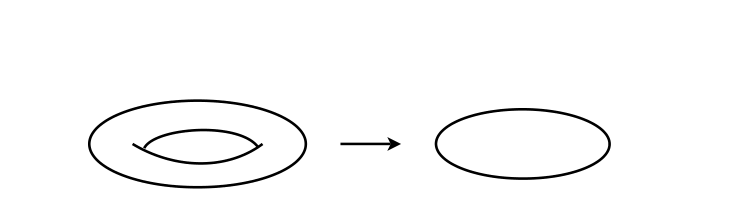
\includegraphics[width=0.4\textwidth]{figures/fig32.2.png}
  \figtitle{32.2}{Gromov--Hausdorff 收敛}
\end{figure}

在这个退化的代数几何模型中，如图 32.1 所示，曲线逐渐被掐细，极限是带结点的有理曲线。另一方面，在 Ricci 平坦的模型中保持直径不变地变形复结构时，则如图 32.2 所示曲线变细，极限是圆周。在代数几何的退化模型中曲率集中的地方，在 Ricci 平坦的模型中几乎是整体。一般地，热带仿射流形对应的不是单个复流形，而是复流形的退化族。

定义依赖于正参数 $t$ 的加法与乘法的变形为
\begin{equation}
x \oplus_t y := -\log_t\left(t^{-x} + t^{-y}\right),\quad x \odot_t y := x + y \tag{32.5}
\end{equation}
则其在 $t \to 0$ 时的极限为
\begin{equation}
x \oplus y := \max\{x,y\},\quad x \odot y := x + y \tag{32.6}
\end{equation}

对收敛 Puiseux 级数环 $\mathbb{K} := \bigcup_{n=1}^{\infty}\C((T^{1/n}))$ 的赋值 $v: \mathbb{K} \to \Q \cup \{\infty\}$ 与绝对值 $|\cdot|: \mathbb{K} \to \R$，对 $x = a_pT^p + a_{p+1/n}T^{p+1/n} + \cdots$（$a_p \ne 0$）定义为 $v(x) = p$ 与 $|x| = \ee^{-p}$。另外，$0$ 的赋值与绝对值分别定义为 $\infty$ 及 $0$。

设 $\boldsymbol{M}$ 为秩 $n$ 的自由 Abel 群，$\boldsymbol{N} := \Hom(\boldsymbol{M}, \Z)$ 为其对偶 Abel 群。对 Laurent 多项式
\begin{equation}
f = \sum_{m \in \boldsymbol{M}} a_m x^{n} \in \mathbb{K}[\boldsymbol{M}] \tag{32.7}
\end{equation}
定义其热带化为
\begin{equation}
f_{\mathrm{trop}}(x) := \max_{m \in \boldsymbol{M}}\left\{v(a_m) + \langle m,x\rangle\right\} \tag{32.8}
\end{equation}
则它确定 $\boldsymbol{N}_{\R} := \boldsymbol{N} \otimes \R$ 上的分片仿射函数，称之为伴随 $f$ 的热带多项式。定义热带多项式 $f_{\mathrm{trop}}$ 所定热带超曲面为
\begin{equation}
V(f_{\mathrm{trop}}) := \left\{x \in \boldsymbol{N}_{\R} \mid f_{\mathrm{trop}} \text{ 在 } x \text{ 处不可微}\right\} \tag{32.9}
\end{equation}
又，置
\begin{equation}
\operatorname{Log} : \boldsymbol{N}_{\mathbb{K}} \to \boldsymbol{N}_{\R},\quad (x_i)_{i=1}^{n} \mapsto (\log|x_i|)_{i=1}^{n} \tag{32.10}
\end{equation}

\begin{theorem}[{[EKL06, Theorem 2.1.1]}]
热带超曲面 $V(f_{\mathrm{trop}})$ 与 $\operatorname{Log}\left(f^{-1}(0)\right)$ 的闭包一致。
\end{theorem}

对正数 $t$，把 Laurent 多项式 $f$ 的系数中出现的 Puiseux 级数的不定元 $T$ 代入 $t$ 所得的 Laurent 多项式记作 $f_t \in \C[\boldsymbol{M}]$。又，置
\begin{equation}
\operatorname{Log}_t : \boldsymbol{N}_{\C}^{\times} \to \boldsymbol{N}_{\R},\quad (z_i)_{i=1}^{n} \mapsto (\log_t|z_i|)_{i=1}^{n} \tag{32.11}
\end{equation}

\begin{theorem}[{[Mik04, Corollary 6.4]}]
关于 $\boldsymbol{N}_{\R}$ 的 Hausdorff 拓扑，
\begin{equation}
\lim_{t \to 0}\operatorname{Log}_t\left(f_t^{-1}(0)\right) = V(f_{\mathrm{trop}}) \tag{32.12}
\end{equation}
成立。
\end{theorem}

\section{Berkovich 空间}

% [Tutor Note: 本节原文以粗体 k 记基域，故此处统一写 \mathbf{k}（preamble 的 \kk 为普通 k，未采用）。]

设 $\mathbf{k}$ 为域。若映射 $v_{\mathbf{k}} : \mathbf{k} \to \R \cup \{\infty\}$ 对任意 $x, y \in \mathbf{k}$ 满足
\begin{enumerate}[label=\arabic*.]
\item $v_{\mathbf{k}}(x) = \infty \Leftrightarrow x = 0$
\item $v_{\mathbf{k}}(xy) = v_{\mathbf{k}}(x) + v_{\mathbf{k}}(y)$
\item $v_{\mathbf{k}}(x+y) \ge \min\{v_{\mathbf{k}}(x), v_{\mathbf{k}}(y)\}$
\end{enumerate}
则称 $v_{\mathbf{k}}$ 为非阿基米德赋值（non-Archimedean valuation）。由非阿基米德赋值，非阿基米德绝对值（non-Archimedean absolute value）$|\cdot|_{\mathbf{k}} : \mathbf{k} \to \R^{\ge 0}$ 由
\begin{equation}
|\cdot|_{\mathbf{k}} = \ee^{-v_{\mathbf{k}}(\cdot)} \tag{33.1}
\end{equation}
确定，而条件 3 被翻译为非阿基米德三角不等式
\begin{itemize}
\item $|x+y|_{\mathbf{k}} \le \max\left\{|x|_{\mathbf{k}}, |y|_{\mathbf{k}}\right\}$
\end{itemize}
域 $\mathbf{k}$ 与其上的非阿基米德绝对值 $|\cdot|_{\mathbf{k}}$ 的组 $(\mathbf{k}, |\cdot|_{\mathbf{k}})$，若非阿基米德绝对值所定的距离 $d(x,y) := |x-y|_{\mathbf{k}}$ 使其完备，则称为非阿基米德域（non-Archimedean field）。

作为复解析几何对非阿基米德域的类似物，有 Tate 的刚性解析空间（Tate's rigid analytic space）[Tat71]、Raynaud 一般纤维（Raynaud generic fiber）[Ray74]、Berkovich 解析空间（Berkovich's analytic space）[Ber90]、Huber 的 adic 空间（Huber's adic space）[Hub93]、藤原--加藤的 Zariski--Riemann 空间 [FK] 等；综述文章可举 [Kat98, Kat03, Con08, Bak08, Tem15, Pay15] 等。以下沿 [KS06]，使用 Berkovich 解析空间。

$\mathbf{k}$ 上的线性空间 $V$ 与映射 $\|\cdot\| : V \to \R^{\ge 0}$ 的组 $(V, \|\cdot\|)$，若对任意 $v, v' \in V$ 与任意 $c \in \mathbf{k}$ 满足
\begin{enumerate}[label=\arabic*.]
\item $\|v + v'\| \le \max\left(\|v\|, \|v'\|\right)$
\item $\|cv\| = |c|_{\mathbf{k}}\|v\|$
\item $\|v\| = 0 \Leftrightarrow v = 0$
\end{enumerate}
则称为 $\mathbf{k}$ 上的 Banach 空间（$\mathbf{k}$-Banach space）。若 $\mathbf{k}$ 上的 Banach 空间 $A$ 具有 $\mathbf{k}$-代数结构，且任意 $a, b \in A$ 满足
\begin{equation}
\|ab\| \le \|a\| \cdot \|b\| \tag{33.2}
\end{equation}
则称 $A$ 为 $\mathbf{k}$ 上的 Banach 代数（$\mathbf{k}$-Banach algebra）。$\mathbf{k}$ 上 Banach 代数 $A$ 的半范数（seminorm）是指满足
\begin{enumerate}[label=\arabic*.]
\item $|0| = 0$
\item $|1| = 1$
\item $|f+g| \le |f| + |g|$
\item $|fg| \le |f|\,|g|$
\end{enumerate}
的映射 $|\cdot| : A \to \R^{\ge 0}$。满足「若 $|f| = 0$ 则 $f = 0$」的半范数 $|\cdot|$ 称为范数。半范数满足 $|fg| = |f|\,|g|$ 时称为乘性的（multiplicative）；半范数满足 $|f| \le \|f\|$ 时称为有界的（bounded）。对 Banach 代数 $A$，在 $A$ 的有界乘性半范数之集合上赋以使映射
\begin{equation}
\mathcal{M}(A) \to \R^{\ge 0},\quad |\cdot| \mapsto |f| \tag{33.3}
\end{equation}
对任意 $f \in A$ 都连续的最弱拓扑，所得空间称为 $A$ 的 Berkovich 谱（Berkovich spectrum），记作 $\mathcal{M}(A)$。

对 $r_1, \dots, r_n > 0$，在
\begin{equation}
\mathbf{k}\left\langle r_1^{-1}X_1, \dots, r_n^{-1}X_n\right\rangle := \left\{\sum_{J} a_J T^J \in K[[X_1, \dots, X_n]] \;\middle|\; |a_J|_{\mathbf{k}}\, r^J \to 0\right\} \tag{33.4}
\end{equation}
上赋以 Gauss 范数
\begin{equation}
\left\|\sum_{J} a_J X^J\right\| := \sup_{J} |a_J|_K\, r^J \tag{33.5}
\end{equation}
所得的 Banach 代数称为变形 Tate 代数（modified Tate algebra）。若 $\mathbf{k}$ 上的 Banach 代数 $A$ 具有从某个变形 Tate 代数出发的满射，且其范数由该变形 Tate 代数的 Gauss 范数诱导，则称 $A$ 为 $\mathbf{k}$-affinoid 代数（$\mathbf{k}$-affinoid algebra）。$\mathbf{k}$-affinoid 代数的 Berkovich 谱称为 affinoid 区域（affinoid domain）。把 affinoid 区域沿适当的 Grothendieck 拓扑黏合所得的空间，称为 Berkovich 解析空间（Berkovich's analytic space）或简称为 Berkovich 空间。存在从 $\mathbf{k}$ 上代数簇的范畴到 Berkovich 空间的范畴、称为解析化（analytification）的函子 $(\cdot)^{\mathrm{an}}$。

定义代数环面 $\mathbb{G}_m^n := \Spec \mathbf{k}[z_1^{\pm 1}, \dots, z_n^{\pm n}]$ 的解析化 $(\mathbb{G}_m^n)^{\mathrm{an}}$ 到 $\R^n$ 的映射为
\begin{equation}
\pi_{\mathrm{can}} : (\mathbb{G}_m^n)^{\mathrm{an}} \to \R^n,\quad x \mapsto (\log|z_1(x)|, \dots, \log|z_n(x)|) \tag{33.6}
\end{equation}
$\mathbf{k}$-代数的层 $\cO^{\mathrm{can}}_{\R^n}$ 由
\begin{equation}
\cO^{\mathrm{can}}_{\R^n}(U) = \left\{f \in \sum_{\omega \in \Z^n} a_\omega z^\omega \;\middle|\; \forall x \in U,\ \lim_{|\omega| \to \infty} \log|a_\omega| + \langle x,\omega\rangle \to \infty = \infty\right\} \tag{33.7}
\end{equation}
定义。

若从 Berkovich 空间到 Hausdorff 空间的映射 $\pi : X \to B^{\mathrm{sm}}$ 满足：对任意 $b \in B^{\mathrm{sm}}$，存在 $b$ 的邻域 $U$ 与 $\R^n$ 的开集 $V$，使图表
\begin{equation}
\begin{array}{ccc}
\pi^{-1}(U) & \xrightarrow{\ \sim\ } & \pi_{\mathrm{can}}^{-1}(V)\\[4pt]
\downarrow & & \downarrow\\[4pt]
U & \xrightarrow{\ \sim\ } & V
\end{array} \tag{33.8}
\end{equation}
交换，则称 $\pi$ 为解析环面纤维化（analytic torus fibration）。其中上行为 Berkovich 空间的同构，下行为同胚。解析环面纤维化的底空间具有这样的热带仿射结构：由
\begin{equation}
\operatorname{Aff}_{\Z,B^{\mathrm{sm}}}(U) := \left\{v(f) + c \mid f \in \cO(\pi^{-1}(U))^{\times},\ c \in \R\right\} \tag{33.9}
\end{equation}
定义的层 $\operatorname{Aff}_{\Z,B^{\mathrm{sm}}}$ 是热带仿射函数构成的层。反之，给定热带仿射流形 $B^{\mathrm{sm}}$ 时，通过黏合 affinoid 区域，可以构造 Berkovich 空间 $X$ 与解析环面纤维化 $\pi : X \to B^{\mathrm{sm}}$。

\begin{question}
$B$ 取 $\R^2$ 的具有热带仿射结构、且在原点有焦点-焦点奇点者。此时，试构造 Berkovich 曲面 $X$ 与连续映射 $\pi : X \to B$，使其在原点之外是解析环面纤维化，并在该处具有给定的热带仿射结构。
\end{question}

此问题由 Kontsevich--Soibelmann 如下解决：首先，把 $(\mathbb{G}_m^{\mathrm{an}})^2$ 的两个副本沿公共部分按
\begin{equation}
\left\{
\begin{array}{rcl}
z'_1 & = & (1+z_2)z_1\\
z'_2 & = & z_2
\end{array}
\right. \tag{33.10}
\end{equation}
黏合，再取部分紧致化，便得到
\begin{equation}
X = \Spec \mathbf{k}[\alpha,\beta,\gamma]/((\alpha\beta-1)\gamma-1) \tag{33.11}
\end{equation}
的解析化 $X^{\mathrm{an}}$。这里 $(\alpha,\beta,\gamma)$ 与 $(z_1,z_2)$、$(z'_1,z'_2)$ 由
\begin{equation}
\alpha = \frac{1}{z_1},\quad \beta = z'_1,\quad \gamma = \frac{1}{z_2} = \frac{1}{z'_2} \tag{33.12}
\end{equation}
相联系。注意由 (33.10) 可得
\begin{align}
v(z'_1) &= v(1+z_2) + v(z_1) \tag{33.13}\\
&= \min\{0, v(z_2)\} + v(z_1) \tag{33.14}\\
&= \begin{cases}
v(z_1) & v(z_2) \ge 0,\\
v(z_1) + v(z_2) & v(z_2) \le 0
\end{cases} \tag{33.15}
\end{align}

\section{$A_1$ 奇点}

镜像由把
\begin{equation}
X = \Spec \mathbf{k}[\alpha,\beta,\gamma]/((\alpha\beta-1)\gamma-1) \tag{34.1}
\end{equation}
与
\begin{equation}
X' = \Spec \mathbf{k}[\alpha',\beta',\gamma']/((\alpha'\beta'-1)\gamma'-1) \tag{34.2}
\end{equation}
按
\begin{equation}
\alpha = \frac{1}{\alpha'},\quad \beta = (\alpha')^2\beta',\quad \gamma = \gamma' \tag{34.3}
\end{equation}
黏合而得。所得空间与把 $\mathbb{A}^2 \setminus \{0\}$ 对 $\mathbb{G}_m$ 的作用 $(z,w,\zeta) \mapsto (\delta z, \delta w, \delta^{-2}\zeta)$ 取商所得的空间
\begin{equation}
K_{\PP^1} \cong \left((\mathbb{A}^2 \setminus \{0\})/\mathbb{G}_m,\right. \tag{34.4}
\end{equation}
的开集通过
\begin{equation}
X \to K_{\PP^1},\quad (\alpha,\beta,\gamma) \mapsto [1,\alpha,\beta], \tag{34.5}
\end{equation}
\begin{equation}
X' \to K_{\PP^1},\quad (\alpha',\beta',\gamma') \mapsto [\alpha',1,\beta'] \tag{34.6}
\end{equation}
同构。

% [Tutor Note: 原文的若干疑似排印问题，均照录图像、未作改动：
%  (a) (32.7) 中 $a_m x^{n}$ 的上标原文印作 $n$（按上下文疑为 $m$）；
%  (b) p046 的 Puiseux 级数环印作黑板的 $\mathbb{K}$，而 p048 的 (33.4)(33.5) 中同一对象
%      印作斜体 $K$；
%  (c) (33.6) 上方 $\Spec \mathbf{k}[z_1^{\pm 1},\dots,z_n^{\pm n}]$ 的末个指数原文印作 $\pm n$
%      （按惯例疑为 $\pm 1$）；
%  (d) (33.7) 中条件原文印作「$\lim_{|\omega|\to\infty}\log|a_\omega| + \langle x,\omega\rangle
%      \to \infty = \infty$」，末尾「$= \infty$」语义重复，照录；
%  (e) (34.4) 的括号在原文中于「$K_{\PP^1} \cong ((\mathbb{A}^2\setminus\{0\})/\mathbb{G}_m,$」
%      处未闭合（下接「の開集合と」），照录；
%  (f) 人名原文作「Kontsevich--Soibelmann」，通行拼写为「Kontsevich--Soibelman」，照录原文。]

% （p049 末尾的「参考文献」标题与首 3 条已由 Lead 并入 c12.tex，此处不再重复。）


% CHUNK c11 DONE pages p043–p049
